% !TEX root = ../intro-stellar-physics.tex

We've established that in the interior of the star a temperature gradient,
\[
	\DD{T}{r} = -\frac{3\rho\kappa_{R}}{4acT^3}\frac{L(r)}{4\pi r^2},
\]
arises to transport heat outward (cf.\ eq.~[\ref{e.gradient-temperature}]).
This gradient becomes steeper as we increases either the flux $L/4\pi r^{2}$ or the mean opacity $\kappa_{\mathrm{R}}$. There is a limit, however, to the magnitude of $|\dif T/\dif r|$; if the gradient is too steep, the warm fluid becomes buoyant relative to the cooler fluid above it and begins to rise. You are familiar with this phenomenon: picture a hot summer day. As the ground absorbs sunlight, it warms the air just above the ground. The warm air rises and forms updrafts. You have perhaps seen hawks riding these updrafts on such a day. Glider pilots also take advantage of these rising thermals to stay aloft. This circulation of fluid induced by a temperature gradient is known as \newterm{convection}. 

You can do a home demonstration of convection.  Brew tea, and pour the hot tea into a saucepan that is on an unlit burner. Use a straw with your thumb over the top to insert a layer of cold milk under the warm tea in the saucepan. The temperature difference between the tea and milk will inhibit their mixing. Light the burner, and watch for the development of convection---you will know it when you see it (Fig.~\ref{f.tea}).

\begin{figure}[htbp]
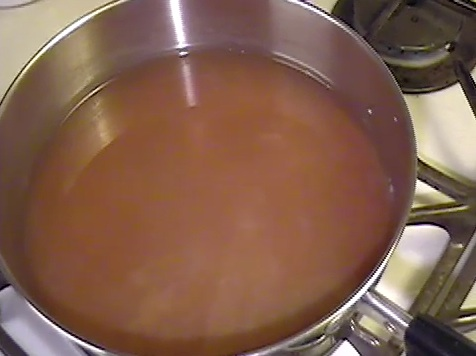
\includegraphics[width=0.5\linewidth]{convection-1}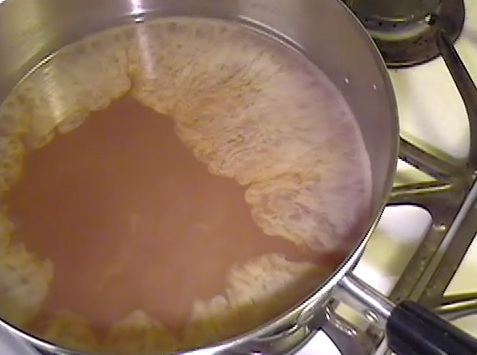
\includegraphics[width=0.5\linewidth]{convection-2}
\caption{Onset of convection in a tea-milk mixture.\label{f.tea}}
\end{figure}

Convection can also occur in stars, in regions of high flux and/or high opacity. During convection, the fluid velocities in question are typically quite subsonic, so we have hydrostatic equilibrium to excellent approximation. But the fluid motions make an enormous difference for heat transport! Warm fluid is carried upward and cool fluid sinks. The net result is that heat is transported upward much faster than it would have been if only diffusion had been operating. This upward transport of heat modifies the temperature gradient. In this chapter, we shall derive the condition for the onset of convection, and the value of the temperature gradient in the presence of subsonic, efficient convective heat transport.

\section{The onset of convection}\label{s.convection-onset}

To understand when convection starts, it helps to recall why a parcel of warm air rises. Recall Archimedes' law:
\begin{quote}\itshape
The buoyant force on an object, either wholly or partially immersed in a fluid under a constant gravitational acceleration, equals the weight of the fluid it displaces.
\end{quote}
What does this mean? A boat of mass $m$ displaces (pushes aside) a volume of water $v$ when floating. The weight of this displaced water, $\rho_{\mathrm{w}}v g$, must equal the weight of the boat $mg$, so that $v = m/\rho_{\mathrm{w}}$.

\begin{marginfigure}
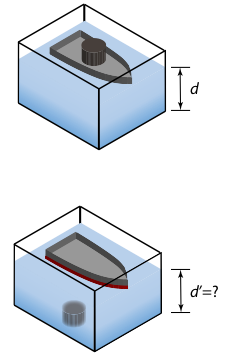
\includegraphics[width=\linewidth]{archimedes}
\caption[A boat with a weight]{\label{f.archimedes} A boat with a weight in a tank. When the weight is tossed overboard and sinks, what happens to the water level in the tank?}
\end{marginfigure}
\begin{exercisebox}[A boat with a weight]
Suppose we have a toy boat carrying a weight and floating in a tank as shown in the top panel of Fig.~\ref{f.archimedes}. The depth of the water in the tank is $d$. The weight is then removed from the boat and allowed to sink to the bottom of the tank (bottom panel, Fig.~\ref{f.archimedes}). Does the depth of water in the tank increase, decrease, or stay the same? Explain your reasoning.
\end{exercisebox}

We can use Archimedes' law---which is an application of hydrostatic equilibrium---to determine whether a fluid in planar geometry and hydrostatic equilibrium,
\begin{equation}
\frac{\dif P}{\dif r} = -\rho g.
\end{equation}
with a temperature gradient is unstable to convection. Imagine moving a blob of fluid upwards from $r$ to $r+h$.  We move the blob slowly enough that it is in hydrostatic equilibrium with its new surroundings, $P_{b}(r+h) = P(r+h)$, where the subscript $b$ refers to ``blob.'' We do move the blob quickly enough, however, that it does not exchange heat with its surroundings and doesn't therefore remain in \emph{thermal} equilibrium with its surroundings. 
\marginnote[-6\baselineskip]{Recall that pressure equilibrium in the blob is established over the time a sound wave takes to cross the blob. Thus, moving the blob slowly enough to maintain pressure equilibrium means that the motion is quite subsonic. Moving the blob quickly enough to prevent heat transport means (cf.\ exercise~\ref{ex.random-walk-diffusion}) that the blob is much larger than a mean free path so the time for photons to random walk across the blob is longer than it takes to lift the blob a distance $h$.}

As a result of this lack of heat exchange, the upward motion of the blob is \newterm{adiabatic}.  To understand what this means, recall the first law of thermodynamics\cite{Fermi1956Thermodynamics}, which relates the change in internal energy $\dif U$ and in volume $\dif V$ to the heat transferred $\dif Q = T\,\dif S$:
\begin{equation}\label{e.first-law-thermo}
	\dif Q = T\,\dif S = \dif U + P\,\dif V,
\end{equation}
where $P$ is the pressure and $S$ is the entropy. During an adiabatic process, $\dif Q = T\,\dif S = 0$. The entropy of the blob\sidenote{We'll use the subscript $b$ to denote properties of the blob; quantities without a subscript refer to the background fluid.} is therefore constant, 
$S_{b}(r+h) = S_{b}(r) = S(r)$, and is therefore not equal, in general, to the entropy of the surrounding gas at $r+h$: $S_{b}(r+h)  \neq S(r+h)$. The pressure in the blob, however, is the same as in the surrounding gas: $P_{b}(r+h) = P(r+h)$.

After the blob has moved from $r$ to $r+h$, it has expanded to occupy a volume
\[
	V_{b}(r+h) = V[P_{b}(r+h),S_{b}(r+h)] = V[P(r+h),S(r)].
\]
Here we've written the volume as a function of pressure and entropy: $V(P,S)$. Now we can apply Archimedes' law: if the volume of the blob is less than the volume occupied by an equal mass of the surrounding fluid, then the buoyant force will be less than the weight of the blob; as a consequence, the blob will sink back to its original location. The fluid is thus stable. In contrast, if the volume occupied by the blob is larger than that occupied by an equivalent mass of the surrounding fluid, then the buoyant force is greater than the weight of the blob; a result, the fluid is unstable, as a small perturbation leads to the acceleration of the blob upwards. Figure~\ref{f.convective-schematic} has a schematic of this criterion.
\begin{marginfigure}
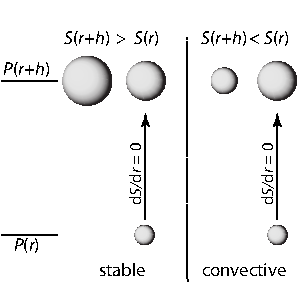
\includegraphics[width=\textwidth]{convective}
\caption[Illustration of criteria for convective instability.]{\label{f.convective-schematic}Illustration of criteria for convective instability.  On the left, raising a blob a distance $h$ adiabatically and in pressure balance with its surrounding results in a higher density $V_{b} < V$.  This is stable: the blob will sink back.  On the right, the blob is less dense and hence buoyant: it will continue to rise.}
\end{marginfigure}

Thus, for the fluid to be stable, we require that the volume of the displaced blob be less than teh volume of an equal mass of surrounding fluid:
\begin{eqnarray}
V_{b}(r+h) &<& V(r+h) \nonumber\\
V[P_{b}(r+h),S_{b}(r+h)] &<& V[P(r+h),S(r+h)] \nonumber\\
V[P(r+h),S(r)] &<& V[P(r+h),S(r+h)].
\label{e.archimedes}
\end{eqnarray}
If condition (\ref{e.archimedes}) is satisfied, then the blob will be restored to its original location after a perturbation, and the system is stable. If condition (\ref{e.archimedes}) is not satisfied, then the blob will continue to rise following a perturbation, and the system is unstable to convection.

Since $h$ is an infinitesimal displacement, we can expand eq.~(\ref{e.archimedes}):
\[
	V[P(r+h),S(r)] < V[P(r+h),S(r+h)] \approx V[P(r+h),S(r)] + \tderiv{V}{S}{P}\DD{S}{r}.
\]
Here the notation $(\partial V/\partial S)_{P}$ means taking the derivative of $V$ with respect to $S$ while holding $P$ fixed. The condition for stability is therefore
\begin{equation}\label{e.convective-stability}
 \tderiv{V}{S}{P}\frac{\dif S}{\dif r} > 0 .
\end{equation}
Changing variables from entropy $S$ to temperature $T$ via
\begin{eqnarray*}
\tderiv{V}{T}{P} &=& \tderiv{V}{S}{P}\tderiv{S}{T}{P}\\
 &=& \frac{C_{P}}{T}\tderiv{V}{S}{P},
 \end{eqnarray*}
 we can rewrite equation~(\ref{e.convective-stability}) as
 \[
 \frac{T}{C_{P}}\tderiv{V}{T}{P}\frac{\dif S}{\dif r} > 0.
 \]
Now, $(\partial V/\partial T)_{P}$ is positive (gas expands on being heated), so our condition for stability is simply
 \begin{equation}\label{e.entropy-condition}
\frac{\dif S}{\dif r} > 0.
\end{equation}
In a convectively stable star, the entropy must increase with radius. if $\dif S/\dif r < 0$, then convection occurs and carries high-entropy material outward, where it will eventually mix with the ambient medium.  As a result, convection drives the entropy gradient toward the marginally stable configuration $\dif S/\dif r = 0$.  If a star is fully convective and mixes efficiently, then the interior of the star lies along an adiabat. 

\section{The adiabatic thermal gradient}\label{s.adiabatic-gradient}

We saw that the temperature gradient in the star is (eq.~[\ref{e.gradient-temperature}])
\[
    \DD{T}{r} = -\frac{3\rho\kappa}{4acT^3}\frac{L(r)}{4\pi r^2}.
\]
Here $\kappa$ is the opacity and $L(r)$ is the luminosity at radius $r$: $L/4\pi r^2$ is the flux. If this thermal gradient, $|\dif T/\dif r|$, becomes too large, however, the fluid becomes unstable: warm fluid begins to rise while cold fluid sinks to take its places.  This usually occurs quickly enough that there is little exchange of heat between the upwelling warm current and the sinking cold one.

Now, we aren't using volume to describe our fluid so let's apply this equation to a fixed mass of fluid, say $m = \val{1}{\kilo\gram}$, and divide both sides of Equation~(\ref{e.first-law-thermo-astro}) by the mass. Then $Q$ refers to the heat transferred \emph{per kilogram}, and $U$ refers to the internal energy \emph{per kilogram}.  Instead of $\dif V$, we then have $\dif(V/m) = \dif(1/\rho) = -\rho^{-2}\dif\rho$.  Our first law, rewritten in terms of mass-specific quantities, is thus
\begin{equation}\label{e.first-law-thermo-astro}
	\dif Q = \dif U -\frac{P}{\rho^{2}}\dif \rho.
\end{equation}
Suppose we wish to express quantities in terms of temperature $T$ and density $\rho$: then
\[ \dif U = \tderiv{U}{T}{\rho}\dif T + \tderiv{U}{\rho}{T}\dif \rho, \]
and
\[ \dif Q = \tderiv{U}{T}{\rho}\dif T + \left[\tderiv{U}{\rho}{T} - \frac{P}{\rho^{2}}\right]\dif \rho. \]
Hence the heat needed to raise the temperature of one kilogram of fluid when holding density fixed is
\begin{equation}\label{e.CV}
C_{\rho} \equiv \tderiv{Q}{T}{\rho} = \tderiv{U}{T}{\rho}.
\end{equation}
For an ideal gas, $U = U(T)$ and $C_{\rho}$ is approximately constant; hence we may integrate equation~(\ref{e.CV}) to obtain $U = C_{\rho}T + \textrm{const}$.

In Eq.~(\ref{e.first-law-thermo-astro}), the last term is $-(P/\rho)\, (\dif\rho/\rho) = -(P/\rho)\,\dif\ln\rho$. This demonstrates a useful trick: take the logarithm of the equation of state, $\ln (P) = \ln(\rho) + \ln (T) + \ln (\kB/\mu\mb)$, and then take the differential to obtain
\[ \frac{\dif P}{P} = \frac{\dif\rho}{\rho} + \frac{\dif T}{T}. \]
Now eliminate $\dif\rho/\rho$ in the equation
\[ \dif Q = C_{\rho}\dif T - \frac{P}{\rho}\frac{\dif\rho}{\rho} \]
to obtain an expression for the heat transferred as a function of temperature and pressure,
\[ \dif Q = \left[C_{\rho} + \frac{P}{\rho T}\right]\dif T - \frac{1}{\rho}\dif P
	 = \left[C_{\rho} + \frac{\kB}{\mu\mb}\right]\dif T - \frac{1}{\rho}\dif P. \]
From this we see that the heat needed to raise the temperature of one kilogram when holding pressure fixed is
\begin{equation}\label{e.CP}
C_{P}\equiv \tderiv{Q}{T}{P} = C_{\rho} + \frac{\kB}{\mu\mb}.
\end{equation}
For a plasma of ions and electrons, $C_\rho = (3/2)\kB/(\mu\mb)$ and hence $C_P = (5/2)\kB/(\mu\mb)$.  The ratio of specific heats is
\begin{equation}\label{e.gamma}
    \gamma = \frac{C_P}{C_\rho} = \frac{5/2}{3/2} = \frac{5}{3}.
\end{equation}
This value of $\gamma$ is for an ideal gas and does not hold universally.

\newthought{During adiabatic motion, there is no heat exchange:} hence, the entropy is constant,
\begin{equation}\label{e.differential-entropy}
    T\dif S = \dif Q = 0 = C_{P}\dif T - \frac{1}{\rho} \dif P.
\end{equation}
Using the ideal gas equation of state we can write 
\[
    \frac{1}{\rho} = \frac{\kB}{\mu\mb} \frac{T}{P}
\]
and insert this into Equation~(\ref{e.differential-entropy}) to obtain
\begin{equation}\label{e.differential-adiabat}
     \frac{\dif T}{T} = \frac{\kB/(\mu\mb)}{C_{P}}\frac{\dif P}{P} = \frac{C_{P}-C_{\rho}}{C_{P}} \frac{\dif P}{P} = \frac{\gamma-1}{\gamma}\frac{\dif P}{P}.
\end{equation}
Integrating both sides of the equation gives
\[ \ln T = \frac{\gamma-1}{\gamma}\ln P + \textrm{const.},\]
or 
\begin{equation}\label{e.adiabat}
 T = T_{0}\left(\frac{P}{P_{0}}\right)^{(\gamma-1)/\gamma},
\end{equation}
where $T_{0}$ and $P_{0}$ are the temperature and pressure at the beginning of the adiabatic process.
Equation~(\ref{e.adiabat}) tells us how the temperature changes with pressure along an adiabat for an ideal gas.  Notice that we can recast Equation~(\ref{e.differential-adiabat}) as
\begin{equation}
    \frac{P}{T}\left(\dd{T}{P}\right)_s = \left(\dd{\ln T}{\ln P}\right)_s = \frac{\gamma-1}{\gamma}.
\label{e.nabla-adiabat}
\end{equation}
Equation~(\ref{e.nabla-adiabat}) tells us how temperature changes with pressure in an adiabatically stratified gas.

\newthought{We can derive a condition for convective stability} in terms of the local gradients of temperature and pressure. Writing $S = S[P(r),T(r)]$ we expand equation~(\ref{e.entropy-condition}) to obtain
\begin{equation}\label{e.schwarzschild-1}
\frac{\dif S}{\dif r} = \tderiv{S}{P}{T} \frac{\dif P}{\dif r} + \tderiv{S}{T}{P}\frac{\dif T}{\dif r} .
\end{equation}
Now, $P$ is a monotonically decreasing function of $r$, which means we can change variables:
\begin{equation}\label{e.TPstar}
\frac{\dif T}{\dif r} = \TPstar \frac{\dif P}{\dif r} .
\end{equation}
Here $\dif T/\dif P|_{\star}$ is the slope of the $T(P)$ relation \emph{for the stellar interior}.  In particular, this is \emph{not} a thermodynamic equality. Substituting equation~(\ref{e.TPstar}) into equation~(\ref{e.schwarzschild-1}), using hydrostatic equilibrium to eliminate $\dif P/\dif r$, and recognizing that $(\partial S/\partial T)_{P} = C_{P}/T$, we obtain
\begin{equation}\label{e.schwarzschild-2}
\frac{\dif S}{\dif r} =  -\rho g\left[\tderiv{S}{P}{T} + \frac{C_{P}}{T} \TPstar \right].
\end{equation}
Finally, we can use the identity
\begin{equation}
\tderiv{S}{P}{T}\tderiv{T}{S}{P}\tderiv{P}{T}{S} = -1
\end{equation}
to simplify equation~(\ref{e.schwarzschild-2}),
\begin{equation}
\frac{\dif S}{\dif r} = -\frac{\rho g}{P}C_{P}\left[\frac{P}{T}\TPstar - \frac{P}{T}\tderiv{T}{P}{S}\right].
 \label{e.schwarzschild}
\end{equation}
Hence, if the term in $\left[\cdot\right]$ is positive, then the fluid is convectively unstable.

Let's use our expression for the flux, Equation~(\ref{e.gradient-temperature}), to put $\left.\dif T/\dif P\right|_\star$ in terms of $\kappa$ and $L(r)$:
\begin{eqnarray}
    \frac{P}{T}\TPstar &=& \frac{P}{T}\DD{T}{r}\DD{r}{P} = \frac{P}{\rho g(r)}\frac{1}{\color{red}T}\frac{{\color{red}3}\rho\kappa}{4c {\color{red}a T^3}}\frac{L(r)}{4\pi r^2} \nonumber\\
    &=& \frac{P}{\color{red}\Prad}\frac{\kappa}{16\pi Gc} \frac{L(r)}{m(r)}.
\end{eqnarray}
The fluid is unstable to convection if
\begin{equation}
    \frac{P}{\Prad}\frac{\kappa}{16\pi Gc}\frac{L(r)}{m(r)} > \tderiv{\ln T}{\ln P}{S}  = \frac{\gamma -1}{\gamma}.
\end{equation}
We have used Equation~(\ref{e.nabla-adiabat}) for the last term here.
This occurs for large $\kappa$ (outer layers of cool stars) or for a high $L(r)/m(r)$ (centers of luminous hot stars).  On the main-sequence, stars with $M \lesssim \Msun$ have convective outer layers; stars with $M \lesssim \val{0.3}{\Msun}$ are fully convective. Stars with $M\gtrsim\Msun$ have convective cores.

\begin{marginfigure}
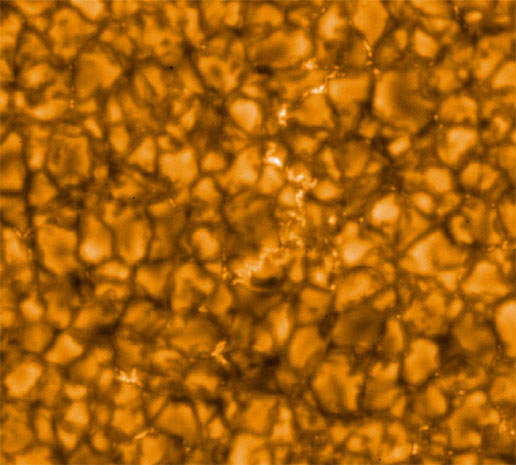
\includegraphics[width=\linewidth]{convection_hinode}
\caption{\label{f.solar-convection]} Solar convection cells, imaged with the Hinode Solar Optical Telescope. Image credit: Hinode JAXA/NASA/PPARC.}
\end{marginfigure}

\begin{exercisebox}[Onset of convection]
The figure shows some hypothetical runs of temperature with respect to pressure in a gas in hydrostatic equilibrium.  Indicate which of these situations is convectively unstable, and explain why. Draw on that plot the pressure-temperature relation that would ensue once convection sets in.

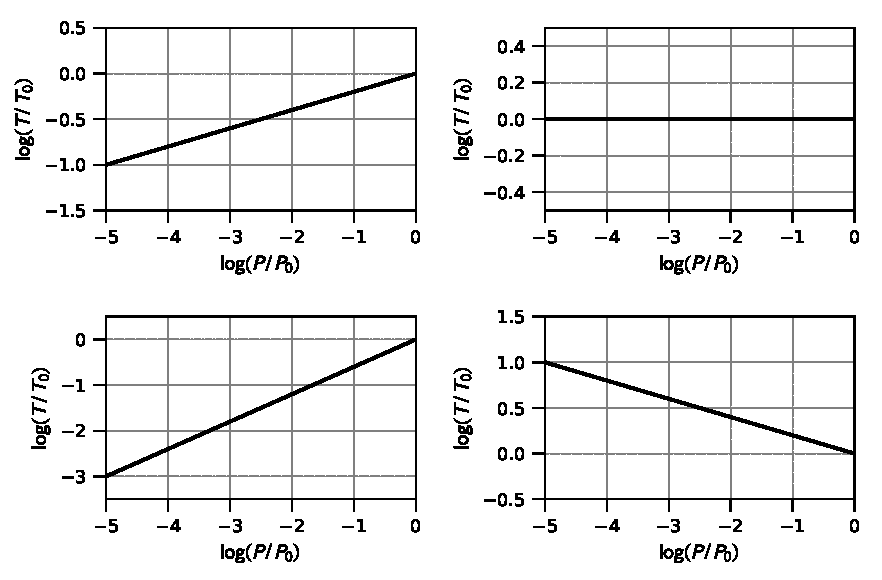
\includegraphics[width=\linewidth]{convection-worksheet-1}
\end{exercisebox}

\begin{exercisebox}[Temperature and density within a star]
The figure below indicates the central density and temperature (\emph{triangle}) for 3 hypothetical stars: (\emph{left}) a star that is fully convective; (\emph{center}) a star with a radiative (i.e., stable against convection) core (densities greater than $\val{10}{\kilo\gram\usk\meter^{-3}}$) and a convective envelope; (\emph{right}) a star with a convective core and a radiative envelope.  For each star, sketch a plausible run of temperature with density within the star. In the center and right panels, the boundary between radiative and convective regions is marked with a vertical solid line.

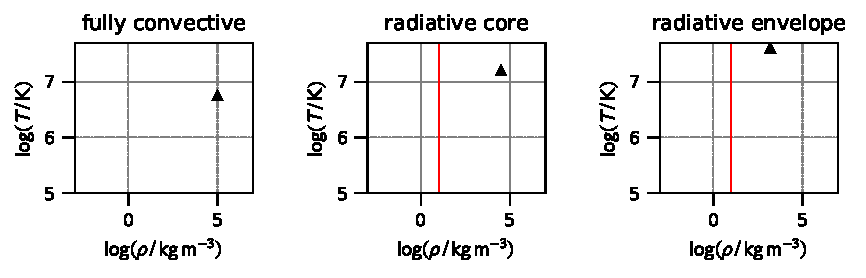
\includegraphics[width=\linewidth]{convection-worksheet-2}
\end{exercisebox}


